\section{Conclusion}


\begin{frame}{Methodological Contributions}
    \begin{itemize}
        \item <1-> A thorough evaluation of Deep Learning Based Content Selection 
            Models
      %  \item Salience Estimation with Deep Learning Content Selection
            \begin{itemize}
    %            \item We show that generic neural architectures are 
    %                just as good as task-specific ones.
                \item We show that neural models are strongly influenced by  position heuristics, especially for news.
            \end{itemize}
        \vspace{5pt}
        \item<2-> Integrated content-focused salience estimation into 2 Stream Summarization Models
            \begin{itemize}
                \item We demonstrate the importance of content-base salience
                    estimation in the stream summarization task.

           %     \item  On stream summarization task, i.e. where position biases are less useful, we demonstrate the importance of content based features
           %     \item We propose two approaches to incorporating a salience estimation model into a stream summarization system.
            \end{itemize}
        \vspace{5pt}
        \item<3-> Noise-injection Sampling and Self-Training Based Data Augmentation
        \begin{itemize}
            \item We demonstrate improved faithfulness in neural NLG models with
                this technique.
%            \item We propose noise-injection sampling and self-training scheme that increases semantic correctness of neural NLG model.
        \end{itemize}
        \vspace{5pt}
        \item<4-> Alignment Training 
        \begin{itemize}
            \item We demonstrate realization order control using this linearization strategy.
%            \item We propose an input transformation to make arbitrary seq2seq models controllable at the of level surface order.
        \end{itemize}
    \end{itemize}
\end{frame}

%\begin{frame}{Contributions}
%    \begin{itemize}
%        \item Salience Estimation with Deep Learning Content Selection
%            \begin{itemize} \tiny
%        \item  Chris Kedzie, Kathleen McKeown, and Hal Daum\'{e} III. \textit{Content Selection in Deep Learning Models of Summarization.} EMNLP 2018.
%            \end{itemize}
%        \item Salience Estimation with Structured Content Selection Models 
%            \begin{itemize} \tiny
%        \item  Chris Kedzie, Kathleen McKeown, and Fernando Diaz. \textit{Predicting Salient Updates for Disaster Summarization.} ACL 2015.
%\vspace{5pt}
%        \item  Chris Kedzie, Fernando Diaz, and Kathleen McKeown. \textit{Real-Time Web Scale Event Summarization Using Sequential Decision Making.} IJCAI 2016.
%            \end{itemize}
%        \item Data Augmentation for Faithful Generation
%        \begin{itemize} \tiny
%        \item Chris Kedzie and Kathleen McKeown. \textit{A Good Sample is Hard to Find: Noise Injection Sampling and Self-Training for Neural Language Generation Models.} INLG 2019.
%        \end{itemize}
%        \item Alignment Training for Controllable Generation
%        \begin{itemize} \tiny
%        \item  Chris Kedzie and Kathleen McKeown. \textit{Controllable Meaning Representation to Text Generation: Linearization and Data Augmentation Strategies.} EMNLP 2020.
%        \end{itemize}
%    \end{itemize}
%\end{frame}


\begin{frame}{Limitations and Future Work}

    \begin{center}
        \resizebox{0.8\textwidth}{!}{
    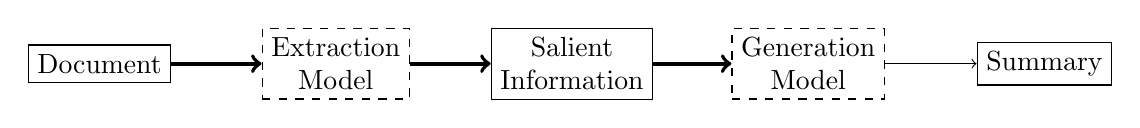
\begin{tikzpicture}
        \node[draw] (doc) at (0,0) {Document}; 
        \node[draw,align=center,dashed] (ext) at (3,0) {{Extraction} \\ {Model}};
        \node[draw,align=center] (cnt) at (6,0) {Salient \\ Information};
        \node[draw,align=center,dashed] (gen) at (9,0) {{Generation} \\ {Model}};
        \node[draw] (sum) at (12,0) {Summary};
        \draw[->,line width=0.5mm] (doc) -- (ext);
        \draw[->,line width=0.5mm] (ext) -- (cnt);
        \draw[->,line width=0.5mm] (cnt) -- (gen);
        \draw[->] (gen) -- (sum);
\end{tikzpicture}}
    \end{center}

\begin{itemize}

\item Contributions up to this point are are focused on pieces of the summarization pipeline in idealized settings.

    \vspace{10pt}
\item Future work needed on mapping extracted content to formal meaning representations suitable for summarization.

    \vspace{10pt}
\item Summarization/Abstraction operations on semantic representations (e.g., AMR) is an interesting and understudied area.

\end{itemize}


\end{frame}

%
%
%\begin{frame}{Contributions}
%
%    \begin{center}
%        \resizebox{0.8\textwidth}{!}{
%    \begin{tikzpicture}
%        \node[draw] (doc) at (0,0) {Document}; 
%        \node[draw,align=center] (ext) at (3,0) {\alert{Extraction} \\ \alert{Model}};
%        \node[draw,align=center] (cnt) at (6,0) {Salient \\ Information};
%        \node[draw,align=center] (gen) at (9,0) {{Generation} \\ \ {Model}};
%        \node[draw] (sum) at (12,0) {Summary};
%        \draw[->] (doc) -- (ext);
%        \draw[->] (ext) -- (cnt);
%        \draw[->] (cnt) -- (gen);
%        \draw[->] (gen) -- (sum);
%%%    \draw[->] (model) -- (sum);
%%%    \uncover<2->{\node[] (tag) at (4,-0.75) {Whats happening in here?};}
%%
%%   
%\end{tikzpicture}}
%    \end{center}
%
%        \textbf{Part I What to say?}
%        \begin{enumerate}
%            \item Salience Estimation with Deep Learning Content Selection
%                    Models
%                    
%                \begin{itemize}
%                    \item Explore several modeling assumptions in neural models of extractive single-document summarization
%                    
%                    \item How to represent sentences?
%
%                    \item How to model salience of sentences w.r.t. document context?
%                    \item Simpler or More generic architecture choices as good as task specific ones.
%                \end{itemize}
%
%        \end{enumerate}
%
%
%\end{frame}
%
%\begin{frame}{Contributions}
%
%    \begin{center}
%        \resizebox{0.8\textwidth}{!}{
%    \begin{tikzpicture}
%        \node[draw] (doc) at (0,0) {Document}; 
%        \node[draw,align=center] (ext) at (3,0) {\alert{Extraction} \\ \alert{Model}};
%        \node[draw,align=center] (cnt) at (6,0) {Salient \\ Information};
%        \node[draw,align=center] (gen) at (9,0) {{Generation} \\ \ {Model}};
%        \node[draw] (sum) at (12,0) {Summary};
%        \draw[->] (doc) -- (ext);
%        \draw[->] (ext) -- (cnt);
%        \draw[->] (cnt) -- (gen);
%        \draw[->] (gen) -- (sum);
%%%    \draw[->] (model) -- (sum);
%%%    \uncover<2->{\node[] (tag) at (4,-0.75) {Whats happening in here?};}
%%
%%   
%\end{tikzpicture}}
%    \end{center}
%
%        \textbf{Part I What to say?}
%        \begin{enumerate}
%            \item[2.] Salience Estimation with Structured Content Selection Models
%                    
%                \begin{itemize}
%                    \item Propose two summarization models for query focused, news-stream summarization.
%%                    
%                    \item SAP model -- salience estimation + clustering
%\only<1>{
%                        \begin{itemize}
%                            \item Combines salience estimation with implicit
%                            frequency information to determine sentence extraction.
%                            \item Identifies important information faster than cluster or prediction based methods alone.
%                        \end{itemize}}
%
%\only<2->{
%                    \item L2S model -- implicitly learn salience estimation 
%                        along with larger summarization task using the Learning-to-Search framework (CITE)
%                        \begin{itemize}
%                            \item Learned policy is a simple linear classifier, works in a greedy, online manner.
%                           \item Identifies information even faster than SAP
%                                 model
%                        \end{itemize}
%
%}
%                \end{itemize}
%        \end{enumerate}
%
%
%\end{frame}
%
%\begin{frame}{Contributions}
%
%    \begin{center}
%        \resizebox{0.8\textwidth}{!}{
%    \begin{tikzpicture}
%        \node[draw] (doc) at (0,0) {Document}; 
%        \node[draw,align=center] (ext) at (3,0) {{Extraction} \\ {Model}};
%        \node[draw,align=center] (cnt) at (6,0) {Salient \\ Information};
%        \node[draw,align=center] (gen) at (9,0) {\alert{Generation} \\ \ \alert{Model}};
%        \node[draw] (sum) at (12,0) {Summary};
%        \draw[->] (doc) -- (ext);
%        \draw[->] (ext) -- (cnt);
%        \draw[->] (cnt) -- (gen);
%        \draw[->] (gen) -- (sum);
%%%    \draw[->] (model) -- (sum);
%%%    \uncover<2->{\node[] (tag) at (4,-0.75) {Whats happening in here?};}
%%
%%   
%\end{tikzpicture}}
%    \end{center}
%
%        \textbf{Part II How to say it?}
%        \begin{enumerate}
%            \item Faithful Generation with Neural NLG models
%                \begin{itemize}
%                    \item Demonstrate failure to generate semantically correct, i.e. faithful, utterances with neural NLG models.
%                    \item Propose a novel Data Augmentation Scheme: Noise-Injection Sampling and Self-Training
%                    \item We demonstrate increased neural NLG model faithfulness when training with data augmentation. 
%                \end{itemize}
%
%        \end{enumerate}
%\end{frame}
%
%\begin{frame}{Contributions}
%
%    \begin{center}
%        \resizebox{0.8\textwidth}{!}{
%    \begin{tikzpicture}
%        \node[draw] (doc) at (0,0) {Document}; 
%        \node[draw,align=center] (ext) at (3,0) {{Extraction} \\ {Model}};
%        \node[draw,align=center] (cnt) at (6,0) {Salient \\ Information};
%        \node[draw,align=center] (gen) at (9,0) {\alert{Generation} \\ \ \alert{Model}};
%        \node[draw] (sum) at (12,0) {Summary};
%        \draw[->] (doc) -- (ext);
%        \draw[->] (ext) -- (cnt);
%        \draw[->] (cnt) -- (gen);
%        \draw[->] (gen) -- (sum);
%%%    \draw[->] (model) -- (sum);
%%%    \uncover<2->{\node[] (tag) at (4,-0.75) {Whats happening in here?};}
%%
%%   
%\end{tikzpicture}}
%    \end{center}
%
%        \textbf{Part II How to say it?}
%        \begin{enumerate}
%            \item[2.] Controllable Generation with Neural NLG models
%                \begin{itemize}
%                    \item Propose Alignment Training input linearization scheme for sequence-to-sequence models.
%                    \item Show that Alignment Training yields neural NLG models capable of following shallow discourse ordering plans. 
%                    \item Improve reliability of control phenomenon with phrase-based data augmentation 
%                \end{itemize}
%
%        \end{enumerate}
%
%
%\end{frame}
%
%\begin{frame}{Thank You for Listening!} 
%
%    \textbf{Papers}
%{ 
%    \begin{itemize}
%        \item \textbf{Part I}
%        \begin{itemize} \tiny
%        \item  Chris Kedzie, Kathleen McKeown, and Hal Daum\'{e} III. \textit{Content Selection in Deep Learning Models of Summarization.} EMNLP 2018.
%\vspace{5pt}
%        \item  Chris Kedzie, Kathleen McKeown, and Fernando Diaz. \textit{Predicting Salient Updates for Disaster Summarization.} ACL 2015.
%\vspace{5pt}
%        \item  Chris Kedzie, Fernando Diaz, and Kathleen McKeown. \textit{Real-Time Web Scale Event Summarization Using Sequential Decision Making.} IJCAI 2016.
%    \end{itemize}
%\vspace{10pt}
%        \item \textbf{Part II}
%        \begin{itemize} \tiny
%        \item Chris Kedzie and Kathleen McKeown. \textit{A Good Sample is Hard to Find: Noise Injection Sampling and Self-Training for Neural Language Generation Models.} INLG 2019.
%\vspace{5pt}
%        \item  Chris Kedzie and Kathleen McKeown. \textit{Controllable Meaning Representation to Text Generation: Linearization and Data Augmentation Strategies.} EMNLP 2020.
%    \end{itemize}
%    \end{itemize}
%}
%\end{frame}
